\documentclass{article}
\usepackage[utf8]{inputenc}
\usepackage{amsmath,amsthm, amssymb}
\usepackage[margin=1in]{geometry}
\usepackage{verbatim}
\usepackage[toc,page]{appendix}
\usepackage[utf8]{inputenc}
\usepackage{geometry}
\usepackage[framemethod=tikz]{mdframed}
\usepackage{indentfirst}
\usepackage{subcaption}
\usepackage{url}
\usepackage{hyperref}
\usepackage{lipsum}
\usepackage{titlesec}
\usepackage[version=3]{mhchem}
\linespread{1.5}
\usepackage{gensymb}
\usepackage{amssymb}
\usepackage{tikz}
\usepackage{tcolorbox}
\usepackage{subcaption}
\usepackage{pgfplots}
\usepackage{mathtools}


\newtcolorbox{mybox}{colback=green!5!white,colframe=green!75!black}


\newtcolorbox{myboxb}{colback=blue!5!white,colframe=blue!75!black}


\newtcolorbox{myboxr}{colback=red!5!white,colframe=red!75!black}



\pgfplotsset{width=7cm,compat=1.9}


\title{Notes from Andrew Ng's course on ML}
\author{hkhurram122}
\date{May 2021}

\begin{document}

\maketitle


\tableofcontents




\newpage


\section{Week 1}


\textbf{What is Machine Learning?}

\textit{ML is the field of making computers learn tasks without explicitly programming them.} - Arther Samuel


\begin{itemize}
    \item This guy gave 1000s of checkers game data to a computer to learn which moves lead to wins against itself, the computer gained so much experience that it became better than Samuel himself.
\end{itemize}



\subsection{Supervised learning}




\subsubsection{Regression Problem}

\begin{mybox}
\textbf{Idea:}
\begin{itemize}
    \item For ex, say that there is some housing data (size vs price). We want to predict the housing price for any arbitrary size. We would then fit the data points with a linear regression line or quadratic fitting.

    \item Supervised means that the right answers were given for every example (actual price to compare with what the algorithm produced).

    \item Regression problem (continuous value problem - price)
\end{itemize}
\end{mybox}



\subsubsection{Classification Problem}

\begin{mybox}
\textbf{Idea:}
\begin{itemize}
    \item Discrete valued output (0 or 1) based on tumer size (for example) - outputs are probabilities that it is one or the other ...
    \item The input could be 1-D, or N-D $\in R$.
    \item For 2D input (2 freatures), the learning algorithm may fit the data with a line to separate the two possible outputs. 
\end{itemize}
\end{mybox}

Infinite number of attributes are possible - by support vector machines!










\subsection{Unsupervised learning}
****

- Data has NO LABELS (no correct answers given)

- The inputs are the only things given for each data points


\textbf{ Clustering algorithm:} used to find structure in the data without knowing the outputs



\par\noindent\rule{\textwidth}{0.4pt}



\textbf{Cocktail party problem:}

Ex: 2 speakers and 2 microphones. Overlapping combination of both speakers voices by each mic. The alg seperates the two voices.

One line of code: 

\begin{verbatim}
    [W,s,v] = svd((repmat(sum(x.*x,1),size(x,1,1).*x)*x');
\end{verbatim}




\subsection{Reinforcement learning, recommender systems} 





\subsection{Model Representation - Linear Regression}


\textbf{m} = Number of training ex

\textbf{x} = input variable (features)

\textbf{y} = output variable (target)

(x, y) - one traingin example


$(x^{i}, y^{i})$ - ith training example 


\textbf{Linear mapping (hypothesis function)}

$h_{\theta} (x)  = \theta_0 + \theta_{1} x$

This is linear regression with one variable 

Univariate linear regression (one vairable input, house size). 

X is the space of input values 

Y is the space of output values 

X = Y = R (the set of reals)

$h: X -> Y$


\subsection{The cost function}

How to choose parameters ($\theta$)??

We wanna make h(x) be as close to y when choosing parameters. 



Minimise:

This \textbf{cost function} is the least square sum cost function

\begin{equation}
    J(\theta_0, \theta_1) = \frac{1}{2m} \sum_{i = 1}^{m} \left(h(x^{i}) - y^{i}  \right)^2
\end{equation}

Finding the thetas so that the funciton above is minimized. We take the square for each example i so that the error isnt negative. 


h(x) is a function of x, for a fixed $\theta$

$J(\theta)$ is a fucntion of the parameter $\theta$



\hspace{}


\begin{mybox}
\textbf{Idea:} In the two variable case (of  adjustable parameters), a contour plot can be used to visualize the cost function for different pairs of $\theta_0$  and $ \theta_1$. The minimum J value corresponds to the best fit to the training data, which means that the sums of the squares of the vertical distances between h(x), the hypothesised output, and the actual, expected output (y) is minimized. 
\end{mybox}


\subsection{Gradient Descent} \label{gradientdescent}

- For an arbitrary $J(\theta_0, \theta_1)$ cost function, not just the mean square error function

- There can be more than 2 parameters in general 


\begin{itemize}
    \item Initialize $\theta$ to a random value
    \item Keep changing parameters to reduce $J$
    \item Until we end up at a minimum 
\end{itemize}


- Take a step in the direction of the gradient $\grad J$. (the direction of steepest descent until reaching a local minimum)

\subsubsection{Gradient descent algorithm}

repeat until convergence 

\begin{equation}
    \theta_j := \theta_j - \alpha \frac{\partial}{\partial \theta_j} J(\theta_0, \theta_1, ...)
\end{equation}


$\alpha$ = Learning rate 


Gradient descent refers to simultaneous update of parameters, where first the updated parameters are computed before they are all updated at the same time.
This is so that the new, computed value of one parameter isn't fed in an updated parameter before it itself is updated to a new value in that iteration.
Different starting points result in different local minima endpoints.


\begin{itemize}
    \item Gradient descent would be small if the learning rate is too small
    \item Gradient descent can overshoot the minimum if the learning rate is too large. May fail to converge, or even diverge.
\end{itemize}


Gradient descent will automatically take smaller steps. So no need to decrease $\alpha$ over time since the derivative becomes smaller as it approaches zero (a local minimum).




\subsection{Gradient Descent for Linear Regression}


Repeat until convergence (

$\theta_0 := \theta_0 - \alpha \frac{1}{m} \sum_{i=1}^m (h_\theta (x_i) - y_i)$

$\theta_1 := \theta_1 - \alpha \frac{1}{m} \sum_{i=1}^m \left( (h_\theta (x_i) - y_i) x_i \right)$

)


These are derived from the multivariate chain rule. And we use the fact that the sum of the derivatives is the derivative of the sum over m training examples, where $j = 1...m$. 






\hspace{}




\textbf{Batch Gradient Descent} : Each step of gradient descent uses ALL of the training examples. 




\subsection{Linear Algebra Review}

\subsubsection{Matrix}
\begin{itemize}
    \item Matrix is a rectangular array of numbers
    \item A 2D array 
    \item Dimension: number of rows x number of columns
    \item $A_{ij} = i,j$ entry 
\end{itemize}

\hspace{}

\subsubsection{Vector}
\begin{itemize}
    \item n x 1 matrix ( one column and many rows )
    \item $\mathbb{R}^4$ is a 4 dimensional vector
    \item $y_i$ is the ith element 
    \item i can start at 0 or 1 
    \item $\textbf{v, w, u} \in V$
\end{itemize}


Using a for loop over matrix multiplication is has a higher time complexity O(n)

Vectorization is more efficient 


\subsubsection{Properties of Matrix Multiplication:}

In general $ A \times B \neq B \times A$
(NOT COMMUTATIVE)


Matrix multiplication IS ASSOCIATIVE 

- refer to medici for properties of a vector space 

- Identity: $I \times A = A$


\subsubsection{Inverse and Transpose}

- Not all numbers have an inverse (0), since 1/0 is undefined

- $A$ is invertible if and only if $A A^{-1} = A^{-1}A = I$. $A$ must be a square matrix. Invertible if it is full row rank and full column rank.



- Transpose: swap the rows and the columns. $B_{ij} = A_{ji}$



\section{Week 2}

\subsection{Multiple Features - Multivariate Linear Regression}

\begin{itemize}
    \item $n$ = number of features
    \item $m$ = number of training examples, rows
    \item $\textbf{x}^{(i)}$ = input vector of features of the $i^{th}$ training example
    \item $x_j^{(i)}$ = value of feature $j$ in the $i^{th}$ training example
\end{itemize}


Hypothesis is trying to predict the price of a house in thousands of dollars:

\begin{equation}
    h_{\theta}(x) = \theta_0 + \theta_1 x_1 + \theta_2 x_2 + ... + \theta_n x_n
\end{equation}



\begin{equation}
    h_{\theta}(x) = {\theta}^T \textbf{x}
\end{equation}

Define $x_0 = 1$ for convenience of notation. The parameters and the feature vector are:

\begin{equation}
    \theta = \begin{pmatrix} \theta_0 \\ \theta_1 \\ ... \\ \theta_n     \end{pmatrix}
     \, \,\, \text{and} \, \, \, \textbf{x} = \begin{pmatrix}
    x_0 \\ x_1 \\ ... \\ x_n
    \end{pmatrix} \in \mathbb{R}^{n+1}
\end{equation}


\subsection{Gradient descent for multiple variables}

The algorithm is: 

repeat until convergence (
\begin{equation}
    \theta_j := \theta_j - \alpha \frac{1}{m} \sum_{i=1}^m \left[ \left(h_{\theta} (x^{(i)}) - y^{(i)}\right) \cdot x_j^{(i)} \right] \, \, \, \text{for } j = 1...n 
\end{equation})

\textit{(loop simultaneously over the number of features there are (equal to number of parameters - 1)}



\subsection{Feature Scaling}


\begin{mybox}{
\textbf{Idea:} Make sure features are on a similar scale, since if they're not, then gradient descent takes a long time, oscillating around until reaching a local minimum.

Make the range of ALL features be \textit{approximately} between $-1 \leq x_i \leq 1$ by dividing all features by the maximum value of that feature in the training set.}
\end{mybox}


Effect: The contours become more circular, rather than skewed (in the 2 parameter case).




\subsection{Mean Normalization}

\begin{mybox}
\textbf{Idea:} Replace $x_i$ with $x_i - \mu_i$ to make the features have approximately zero mean (centered at 0) 

We can use the formula to normalize $x_i$ (features where i = 1...n, NOT when i = 0 since $x_0 = 1$ over all training data):

\begin{equation}
    x_i := \frac{x_i - \mu_i}{s_i}
\end{equation}

Where $\mu_i$ is the average value of $x_i$ inn the training set. $s_i$ can be the \textbf{range} or the \textbf{standard deviation}.
\end{mybox}







\subsection{Learning Rate}


\begin{center}

\textbf{Debugging gradient descent} Sample plot of $J$ against the number of iterations:

    \begin{tikzpicture}
    \draw[->] (-1,0) -- (4.2,0) node[right] {number of iterations};
    \draw[->] (0,-1) -- (0,4.2) node[right] {$\underset{\theta}{min}J(\theta)$};
    \draw[scale=0.7, domain=0:5, smooth, variable=\x, blue] plot ({\x}, {5*exp{-\x}});
    \end{tikzpicture}
\end{center}


\textbf{Automatic convergence test:} Declare convergence if $J(\theta)$ decreases by less than $\epsilon = 10^{-3}$ in one iteration.

\hspace{}

\begin{myboxb}
\textbf{Theorem?:} For sufficiently small $\alpha$, $J$ should decrease on every iteration.

If J increases with number of iterations progressing, then you should decrease the learning rate.


Try: $\alpha = ..., 0.001, ... , 0.01, ... , 0.1, ...,  1, ...$
\end{myboxb}


\subsection{Features and Polynomial Regression}

\begin{enumerate}
    \item We can combine multiple features into one
    \item We can create new features such as $x_2 = x_1^2$ and $x_3 = x_1^3$.
\end{enumerate}



\subsection{Normal Equation}

Method to solve for $\theta$ analytically, or directly instead of iteratively, as was seen for gradient descent (\ref{gradientdescent}).


\begin{mybox}
    \textbf{Idea:}
    
    Let $J(\theta) = a\theta^2 + b \theta + c$
    
    Take the derivative and set it to zero to find the minimum: 
    
    $\frac{d}{d\theta} J(\theta) = ... = 0$ and solve for $\theta$.
\end{mybox}


\begin{mybox}
    But $\theta \in \mathbb{R}^{n+1}$ is a vector, so how do we minimize $J(\theta)$ in terms of all the $\theta_i$ where $i= 0 ... m$?
    
    The method involves a derivation from ESC103.
    
    Minimize $J$ by explicitly taking its derivatives wrt the $\theta_j$'s and setting them to zero using the formula involving matrices:
    
    \begin{equation}
        \theta = \left(X^T X \right)^{-1} X^T \textbf{y}
    \end{equation}

    Where,
    
    \begin{equation}
        X = \begin{pmatrix}
            1 && x_1^{(1)} && x_2^{(1)} && ... && x_n^{(1)} \\
            ... \\
            1 && x_1^{(m)} && x_2^{(m)} && ... && x_n^{(m)}
        \end{pmatrix}
        \, \, \, \text{and} \, \, \, 
        \begin{pmatrix}
            y^{(1)} \\
            ... \\ 
            y^{(m)}
        \end{pmatrix}
    \end{equation}
\end{mybox}



\begin{table}[h]
\centering
\begin{tabular}{ll} 
\hline
\multicolumn{1}{|l|}{\textbf{Gradient Descent}}  & \multicolumn{1}{l|}{\textbf{Normal Equation}}  \\ 
\hline
Need to choose alpha                             & No need to choose alpha                        \\
Needs many iterations                            & No iterations (one step)                        \\
$\mathcal{O}(kn^2)$                                       & $\mathcal{O}(n^3)$ to calculate the matrix inverse      \\
Works well when n is large (greater then 10,000) & Slow if n is very large (greater than 10,000) 
\end{tabular}
\end{table}


- Feature scaling is not needed with the normal equation.

\hspace{}

- But what if $X^T X$ is non-invertible?? Why?


\begin{itemize}
\item \textbf{There may be redundant features:}
 Non invertible when one feature can be expressed as a linear combination of other features (\textbf{linearly dependent}), then the dimension of the column (and row space) is less than the number of columns there are, so the product wouldn't be full rank and thus singular.
\item \textbf{Small data and large number of features} may also cause non-invertibility (short and wide). Delete some features or use regularization.
\end{itemize}



\section{Week 3}

\subsection{Classification}


The output is a discrete value, $y \in {0, 1}$, where $0$ is the Negative class and $1$ is the Positive case.


\begin{myboxr}
If we try to apply linear regression $h_{\theta} (x) = \theta^T \textbf{x}$, then we can threshold the classifier output $h_{\theta} (x)$ at 0.5:

\begin{itemize}
    \item if $h(x) \geq 0.5$, predict "y=1"
    \item if $h(x) < 0.5$, predict "y=0"
\end{itemize}

The $h$'s that result would be inaccurate if a training example is much larger than the rest of the data. The linear $h$ straight line fit constrained by the thresholds would thus NOT be accurate. 

\end{myboxr}


Logistic Regression: $0 \leq h_{\theta} (x) \leq 1$ is a classification algorithm


\subsubsection{Hypothesis Representation}

\begin{equation}
    h_{\theta} = g(\theta^T \textbf{x})
\end{equation}

Where,
\begin{equation}
    g(z) = \frac{1}{1+e^{-z}}
\end{equation}

\begin{center}
    \begin{tikzpicture}
    \draw[->] (-4.2,0) -- (4.2,0) node[right] {z};
    \draw[->] (0,-0.2) -- (0,1.2) node[right] {$g(z)$};
    \draw[scale=0.7, domain=-5:5, smooth, variable=\x, blue] plot ({\x}, {1/(1+exp{-\x})});
    \end{tikzpicture}
\end{center}


We need to fit the parameters $\theta$.

$h(x) =$ estimated probability that y = 1 on input $\textbf{x}$. There is only one output  'neuron'.

\begin{equation}
    h_{\theta} (\textbf{x)} = P(y = 1  \mid \textbf{x}; \theta)
\end{equation}

"probability that y = 1, given \textbf{x}, parameters by $\theta$."


\begin{equation}
    P(y = 1 \mid \textbf{x};\theta) = 1 - P(y=1 \mid \textbf{x}; \theta)
\end{equation}




\subsubsection{Decision Boundary}

The line that separates the region of $x_0, x_1, ...$ plane of inputs $nth-$dimension, where the hypothesis predicts $y=1$ from the region where the hypothesis predicts $y=0$.

The decision boundary is a property of the hypothesis once we've found the optimal $\theta$'s included in the function $h_{\theta} (x)$. Even if we take away the training data ($\textbf{x}$), the decision boundary remains the same. Determining the $\theta$ values however does depend on the training set.

There are also non-linear decision boundaries. We can add higher order terms to $z$ (powers of the input features, $x_i$), and setting $z = 0$ to obtain the decision boundary.


\subsection{Cost Function in Logistic Regression (classification)}

\begin{myboxr}
First, consider using the MSE function used previously as linear regression's cost function.

\begin{equation}
    h_{\theta} (x) = \frac{1}{1+e^{-\theta^T x}}
\end{equation}



\begin{equation}
    J(\theta) = \frac{1}{m} \sum_{i=1}^{m} \frac{1}{2} \left(h_{\theta} (x^{(i)}) - y^{(i)}\right)^2
\end{equation}


Where,
\begin{equation}
    Cost(h_{\theta} (x), y) = \frac{1}{2} \left( h_{\theta} (x) - y \right)^2
\end{equation}

and

\begin{equation}
    h_{\theta} (x) = \frac{1}{1 + e^{-\theta^T x}}
\end{equation}


But the problem here is that the mean square error cost function results in a non-convex function, one that does not have a clear, single local minima that gradient descent can converge to. 

\end{myboxr}



\begin{mybox}
    \textbf{Idea:} Hence, we use the \textbf{logistic regression cost function }to have a CONVEX function.

    
    \begin{equation}
        J(\theta) = \frac{1}{m} \sum_{i=1}^{m} Cost \left(h_{\theta} (x^{(i)}), y^{(i)}\right)
    \end{equation}


    For a \textbf{\textit{single training example,}} the cost function is (also graphed below):
    \begin{equation}
        Cost \left(h_{\theta} (x^{(i)}), y^{(i)} \right) = \left\{
        \begin{array}{ll}
        -log \left(h_{\theta} (x) \right) & \text{ if } y = 1 \\
        -log \left(1 - h_{\theta} (x) \right) & \text{ if } y = 0
        \end{array} \right.
    \end{equation}
    
    
    
    
    
    
    
    \begin{tikzpicture}
        \begin{axis}[
            axis lines = left,
            xlabel = $h_{\theta} (x)$,
            ylabel = $Cost(h_{\theta})$,
        ]
        \addplot [
            domain=0:1, 
            samples=100, 
            color=red,
        ]
        {-ln(x)};
        \addlegendentry{$y = 1$}
        \end{axis}
    
    \end{tikzpicture}
    \hskip 5pt
    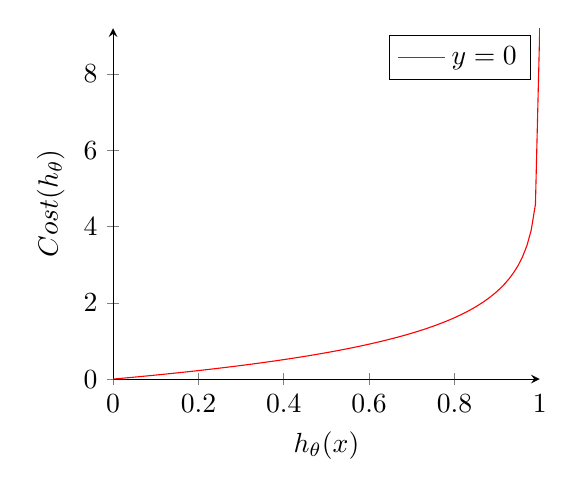
\begin{tikzpicture}
        \begin{axis}[
            axis lines = left,
            xlabel = $h_{\theta} (x)$,
            ylabel = $Cost(h_{\theta})$,
        ]
        \addplot [
            domain=0:1, 
            samples=100, 
            color=red,
        ]
        {-ln(1-x)};
        \addlegendentry{$y = 0$}
        \end{axis}
    
        
    \end{tikzpicture}

        
    
    
    
\end{mybox}




\subsubsection{Simplified cost function and gradient descent}
$y=0$ or $1$ always, so the following is equivalent to equation 18:

\begin{equation}
    Cost \left (h_{\theta} (x), y \right) = -y log(h_{\theta} (x)) - (1-y) log \left( 1- h_{\theta} (x) \right)  
\end{equation}

Principle of maximum likelihood estimation in statistics derives this cost function (for a single training example). 


To fit parameters $\theta$:

\begin{equation}
    \underset{\theta}{min} J(\theta) \text{... Get } \theta 
\end{equation}

The output of the hypothesis is the probability that $y=1$.

\newpage

\subsubsection{Gradient Descent Algorithm}


\begin{equation}
    \frac{\partial}{\partial \theta_j} J(\theta) = \frac{1}{m} \sum_{i=1}^m \left(h_{\theta} (x^{(i)})- y^{(i)} \right) x_j^{(i)}
\end{equation}


\begin{myboxb}
The learning algorithm is this:

Repeat(

$\theta_j := \theta_j +\alpha \cdot  \frac{1}{m} \sum_{i=1}^m \left(h_{\theta} (x^{(i)})- y^{(i)} \right) x_j^{(i)}$ 
 
 
) (simultaneously update all $\theta_j$)

\end{myboxb}





Even though this is the same update rule as in linear regression, the hypothesis function has now changed to a logistic, sigmoid function!



Implementation:  we can use a for loop from i = 0 to n, but a vectorized method is better to update all the thetas.

\begin{figure}[h]
    \centering
    \includegraphics[width=9cm,height=9cm,keepaspectratio]{Screen Shot 2021-05-23 at 8.04.25 PM.png}
    \caption{Vectorized Implementation for computing h and the cost function over all m training examples}
    \label{fig:my_label}
\end{figure}


\begin{figure}[h]
    \centering
    \includegraphics[width=7cm,height=7cm,keepaspectratio]{Screen Shot 2021-05-23 at 8.10.04 PM.png}
    \caption{Vectorized Implementation for simultaneously updating the thetas}
    \label{fig:my_label}
\end{figure}




\subsubsection{Advanced Optimizaton}

Optimization algorithms that can use the values of $J(\theta)$ and $\frac{\partial}{\partial \theta_j} J(\theta)$:
\begin{itemize}
    \item Gradient descent
    \item Conjugate gradient
    \item BFGS
    \item L-BFGS
\end{itemize}

Other algorithms automatically pick a learning rate. Others are often faster than gradient descent. Disadvantages: more complex




\subsubsection{Multi-class Classification: One vs all}


This is basically where we have multiple outputs, or categories we want to predict the probability for each in with h(x), which outputs a vector of said probabilities. Eg. Medical diagrams: Not ill, cold, flu.


How is the decision boundary determined (with the optimal thetas where the cost is minimized)???

- We basically set each class against all other classes. We create a new training set where say, class 1 is set to the positive case (y=1), and class 2,3,4,... are set to be negative cases (y=0). $h$ is a vector where the decision boundary is differnt for each class.


\begin{equation}
    h_{\theta}^{(i)} = P \left(y=i \mid x; \theta \right) \text{ where } (i= 1,2,3,4,...)
\end{equation}


We need to train a logistic regression classifier $h$ for each class $i$ to predict that $y=i$

On a new input $x$, to make a prediction we pick the class $i$ that maximizes the probability predicted for that particular $i$, so:

\begin{equation}
    prediction = \underset{i}{max}  h_{\theta}^{(i)} (x)
\end{equation}




\subsection{The problem of over-fitting - Regularization}

\textbf{Overfitting:} If we have too many features, the learned hypothesis may fit the training set very well, but fail to generalize to new examples (predict prices on NEW examples)



Addressing overfitting:
\begin{itemize}
    \item Reduce the number of features - Manually select which features to keep, or use Model selection algorithms
    \item Regularization - Keep all the features, but reduce the magnitude of parameters $\theta_j$, Works well when we have a lot of features, each of which contributes a bit to predicting $y$
\end{itemize}


\subsubsection{Regularization Cost Function}

Suppose we penalize and make $\theta_3, \theta_4$ really small in the quartic fit to data that is supposed to be overfitting the sample training data, using the objective function:

\begin{equation}
    \underset{\theta}{min} \frac{1}{2m} \sum_{i=1}^{m} \left(h\theta (x^{(i)} - y^{(i)} \right)^2 + 1000 \theta_3^2 + 1000 \theta_4^2
\end{equation}

Results in a "simpler" hypothesis, and is less prone to overfitting (curve is more smoother)



\begin{mybox}

\textbf{General Idea: } But say if there are 100 features, it is hard to decide which features to reduce in magnitude. Solution is to shrink ALL of the parameters from $i = 1...100$ (do not penalize $\theta_0$) :


\begin{equation}
    J(\theta) = \frac{1}{2m} \left[ \sum_{i=1}^m ( h_{\theta} (x^{(i)} - y^{(i)})^2 + \lambda \sum_{j=1}^n {\theta_j}^2 \right]
\end{equation}

\begin{center}
\textit{(linear regression cost function)}
\end{center}

$\lambda$ is the regularization parameter. It controls the tradeoff between fitting the data well (first sum term) and the second sum term, which serves to reduce overfitting.


\end{mybox}



\begin{myboxr}

\textit{What if $\lambda$ is set to an extremely large value (say $\lambda = 10^{10}$)?}

\begin{itemize}

    \item Then we end up with all $\theta_j = 0$ for all $j = 1 ... n$. This is equivilent to eliminating all of the parameters except $\theta_0$. 
    
    \item The hypothesis has too high a bias as $h_{\theta} (x) = \theta_0$ which is just a flat horizontal line, (underfitting).
\end{itemize}

\end{myboxr}


\subsubsection{Regularized Linear Regression}



\textbf{Gradient Descent Algorithm}

Repeat (
    
    $\theta_0 := \theta_0 - \alpha \frac{1}{m} \sum \left(h_{\theta} (x^{(i)} - y^{(i)}) x_0^{(i)} \right)$
    
    $\theta_j := \theta_j (1 - \alpha \frac{\lambda}{m}) - \alpha \frac{1}{m} \sum \left(h_{\theta} (x^{(i)} - y^{(i)}) x_j^{(i)} \right)$
    
)


\par\noindent\rule{\textwidth}{0.4pt}


\textbf{Using the normal equation:}

\begin{equation}
    \theta = \left( X^T X + \lambda \begin{bmatrix} 
    0&&& \\
      &1&& \\
      &&\ddots& \\
      &&& 1 \end{bmatrix} \right)^{-1} X^T y
\end{equation}




\subsubsection{Regularized Logistic Regression}

\begin{verbatim}
function = [jVal, gradient] = costFunction(theta)


%compute the cost value
\end{verbatim}


\begin{equation}
   J(\theta) = \left[ - \frac{1}{m}  \sum_{i=1}^m  \underbrace{y^{(i)} log(h_{\theta} (x^{(i)})) + (1-y^{(i)}) log \left( 1- h_{\theta} (x) \right) }_\textrm{unregularized part of cost - to increase fit to training data} \right] + \underbrace{\frac{\lambda}{2m} \sum_{j=1}^n \theta_j^2}_\textrm{regularization part}
\end{equation}

\begin{verbatim}
gradient(1) = 

gradient(2) = 
\end{verbatim}
\begin{equation}
\frac{\partial J(\theta)}{\partial \theta_j} = \left( \frac{1}{m}\sum_{i=1}^m{\left( h_\theta(x^{(i)})-y^{(i)}\right)x_j^{(i)}} \right)+\frac{\lambda}{m}\theta_j\qquad \mathrm{for}\;j\geq1
\end{equation}

\begin{verbatim}
...
\end{verbatim}






\section{Week 4}

\subsection{Non-linear Hypotheses - Neural Networks}

Problems involving non-linear hypothesis functions.


The number of total features for 2nd order features grows as $O(n^2)$. For 3rd order feature terms in the hypothesis, it grows as $O(n^3)$... So the original function $h$ with arbitrary number of powers used is not feasible for large $n$, the number of original features from the data collected.


\subsubsection{Motivation for Neural Newtorks:}

Take the example of an image classifier that determines whether a given image is of a car or not.

The dimension of the input data, $\textbf{x}$, or feature vector, is an n-th dimensional vector that contains n features which are pixels. The One-versus all principle for determining the non-linear decision boundaries between one pixel vs all others applies.

Say there are 50x50 = 2500 pixels. If a hypothesis function were to consist of non-linear, quadratic terms (all product combinations of features (pixels) that are 2nd order or $(x_i \times x_j)$), there would be 3 million features (terms in the hypothesis function). It again grows as $O(n^2)$.


\subsection{Neural Networks}

The "one learning algorithm" hypothesis:

- Auditory cortex learns to see if hearing is blocked with that nerve and replaced by rewiring. Neuro-rewiring on different parts of the brain suggest that there is a common underlying algorithm in the brain tissue in all parts since any part of the brain can learn to "see". We don't need different programs to make different sensory functions work, one common learning algorithm will do! This is also related to the brains neuro-plasticity!



\subsubsection{Model Representation I}

Biological neuron in the brain:

\begin{itemize}
    \item Dendrite: "input wires"
    \item Cell body containing the nucleus
    \item Axon: The output wire that sends messages to other neurons. Said "messages" are electical pulses that link to the dendrites of other neurons.
\end{itemize}


\textbf{Artificial Neural Network: Logistic unit}

Sigmoid activation function that applies the non-linearity:
\begin{equation}
    h_{\theta} (x) = \frac{1}{1 + e^{-\theta^T x}}
\end{equation}

This is the function that computes the output. 

\begin{itemize}
\item $x_0$ is the bias term. (skim IA, this has been learned before). 

\item $a_{i}^{(j)} =$ activation of unit i in layer j

\item $\Theta^{(i)}$ is a matrix of weights that controls the mapping from layer $j$ to layer $j+1$. $\Theta^{(i)} \in \mathbb{R}^{s_{j+1} \times  (s_{j} + 1)} $, where the +1 comes from the bias term applied to each neuron in layer $j+1$.
\end{itemize}



\subsubsection{Model Representation II}

\begin{figure}[h]
    \centering
    \includegraphics[width=7cm,height=7cm,keepaspectratio]{Screen Shot 2021-05-28 at 6.54.15 PM.png}
    \caption{Neural Network}
    \label{fig:my_labelneural}
\end{figure}


Vectorized implementation of neural networks to learn non-linear hypotheses. Forward propagation is as follows:


\begin{equation}
    \textbf{z}^{(2)} = \Theta^{(1)} \textbf{a}^{(1)}  \text{ where } \textbf{a}^{(1)} \in \mathbb{R}^{4 \times 1}
\end{equation}
\begin{equation}
    \textbf{a}^{(2)} = g \left( \textbf{z}^{(2)} \right)
\end{equation}

Adding the bias term $a_{0}^{(2)} = 1$, whereby $\textbf{a}^{(2)} \in \mathbb{R}^{4 \times 1}$


\begin{equation}
    \textbf{z}^{(3)} = \Theta^{(2)} \textbf{a}^{(2)}
\end{equation}
\begin{equation}
    h_{\Theta}(x) = a^{(3)} = g(\textbf{z})
\end{equation}


Neural networks (with sigmoid activations) are the same as logistic regression algs but where the features fed into logistic regression are themselves the outputs of functions learned in the previous layer, by another set of features. So neural networks create new features for every additional hidden layer involved, accounting for the non-linearity, and the network itself determines what features to use by adjusting weights. The features' selection is itself learned by the NN itself, and is more flexible than using the features $x_i$ themselves or even polynomial terms of $x$.


\subsubsection{Examples and Intuitions}

Non-linear classification example, XOR/XNOR where $x_1$ and $x_2$ are binary (0 or 1)

$y = x_1 XOR x_2$ (true only if one of $x_1$ or $x_2$ are true)

$x_1 XNOR x_2$, which is $NOT \, (x_1 XOR x_2)$ (true only if both are true or both false)


Negation: $NOT x_1$


\par\noindent\rule{\textwidth}{0.4pt}

\subsubsection{Multiclass Classification}

Extension of the one-vs-all algorithm

We need $p$ neurons in the output layer of the neural network, each which represents the probability that the image is of one category out of $p$ categories, or labels.


\section{Week 5}


\subsection{Cost Function with Neural Nets}

In binary classification, the number of output units, $s_j$ for $j=L$ (where $L$ is the number of layers in the NN), is 1, which is the probability that the example $x^{(i)}$ corresponds to the $y=1$ case.

In multiclass classification, the hypothesis results in a $R^{K \times 1}$ column vector that represents the probabilities that a given example (set of features) is a certain class. 

\begin{mybox}

Logistic Regression:
\begin{equation}
    J(\theta) = -\frac{1}{m} \left[ \sum_{i=1}^m y^{(i)} log h_{\theta} (x^{(i)}) + (1-y^{(i)})log(1 - h_{\theta} (x^{(i)})) \right] + \frac{\lambda}{2m} \sum_{j=1}^n \theta_j^2
\end{equation}

Neural Network:
\begin{equation}
    J(\Theta) = - \frac{1}{m} \left[ \sum_{i=1}^m \sum_{k=1}^K y_k^{(i)} log \left(h_{\Theta} (x^{(i)})\right)_k + \left(1 - y_k^{(i)} \right) log \left(1 - (h_{\Theta} (x^{(i)}))_k \right) \right] + \frac{\lambda}{2m} \sum_{l=1}^{L-1} \sum_{i=1}^{s_l} \sum_{j=1}^{s_{l+1}} (\Theta_{ji}^{(l)})^2
\end{equation}

Notes:
\begin{itemize}
    \item We don't regularize the $\theta_{ij}$ where $i=0$ since that corresponds to the weight associated with the bias unit.
    \item When trying to minimize $J(\Theta)$ using the advanced optimization algorithms, the function pointer that we pass on should point to a function f, that returns the value of $J$ (cost) and the partial derivatives for every $i, j, l$.
\end{itemize}

\end{mybox}








\subsection{Backpropagation Algorithm}

Intuition: $\delta_j^{(l)}$ = "error" of node j in layer l which is $\delta_j^{({4})} = a_j^{(4)} - y_j$ if the output layer is denoted as layer 4. 3

The errors of the previous layer nodes is derived from the chain rule.

\begin{myboxb}
    
    
\textbf{Pseudocode (MATLAB type) algorithm implementation of Backprop:} 

Given a training set $\{ (x^{(1)}, y^{(1)}) ... (x^{(m)}, y^{(m)}) \}$

\begin{verbatim}
    Delta(i, j, l) = 0 % for all l i j (for a full matrix of zeroes)
    
    for t = 1:m, % loop over all the training examples
        a(1) = X(t)
        
        z(2) = Theta(1) * a(1)
        a(2) = sigmoid(z(2))
        a(2) = [a(0,2) ; a(2)] % add a bias neuron
        ...
        h = sigmoid(z(L-1)) % L is the number of layers
        
        
        delta(L) = a(L) - y(t) % error term for the last layer
        
        delta(L-1) = 
        delta(L-2) = 
        ...
        delta(2) = 
        
        % we don't update delta(1) since we 
        % aren't gonna change the input data with the gradient 
        
        % Use: delta(l) = ((Theta(l))' * delta(l+1)).* a(l) .* (1 - a(l))
        
        Delta(l) = Delta(l) + delta(l+1) * (a(l))'
        
    % now we update our new Delta matrix of all the parameters
    if j != 0: D(i, j, l) = (1/m) * (Delta(i, j, l) + lambda * Theta(i, j, l)) 
    elif j == 0: D(i, j, l) = (1/m) * (Delta(i, j, l) 
    
\end{verbatim}
\end{myboxb}


Here above, $ \frac{\partial}{\partial \Theta_{ij}^{(l)}} J(\Theta) = D_{ij}^{(l)} $, which is the step we take for all $\Theta$ in the neural network.

\begin{equation}
    \Delta_{ij}^{(l)} := \Delta_{ij}^{(l)} + a_j^{(l)} \delta_i^{(l+1)}
\end{equation}



\subsubsection{Backpropagation Intuition}

$\delta_j^{(l)}$ is the error of the cost for a neuron $a_j^{(l)}$ (unit j in layer l)

Formally, 

\begin{equation}
    \delta_j^{(l)} = \frac{\partial}{\partial z_j^{(l)}} cost (i) \text{for } j \geq 0
\end{equation}

\begin{equation}
    cost(i) = y^{(i)} log(h_{\Theta} (x^{(i)}) + (1 - y^{(i)}) log(h_{\Theta} (x^{(i)}))
\end{equation}

The error term is used to change, or update the weights so that the intermediate neurons (z) all change so that the cost is minimized during training by the chain rule tree method starting from the output neuron.


\subsection{Implementation of NN: Forward prop and backprop}

\begin{myboxr}
Note: You cannot initialize $\Theta$ with zero entries when using neural networks. You end up with the same activations on the neurons, the same $\delta_i^{(l)}$, and the same partial derivatives of $J(\Theta)$ wrt to all of the $\Theta_{ij}^{l}$. Hence the all the weights in the same layer starting from the same neuron will remain the same. After each update, parameters corresponding to the inputs going into each of the $s_{l+1}$ hidden units are identical.
\end{myboxr}

\begin{mybox}
\textbf{Implementation:} Random initialization is used for symmetry breaking. 

Initialize each theta to a random value in $[- \epsilon, \epsilon]$.

\end{mybox}



\begin{enumerate}
    \item Randomly initialize weights
    \item Implement forward prop to get h for any x(i)
    \item Implement code to compute the cost function
    \item Implement backprop to compute partial derivatives
    \item Loop through all the training examples and perform forward prop and backprop using example (x(i), y(i))
        (get activations a(l) and delta terms for l = 2 ... L)
        
    \item Use gradient checking to compute the partial derivatives (numerical estimate of $J(\Theta)$. Then disable gradient checking code.
    \item Use gradient descent or an advanced optimization method with back-propagation to try to minimize $J(\Theta)$ as a function of parameters $\Theta$. $J(\Theta)$ is however non-convex, so we can't guarantee that the local minimum we converge to is the global minimum.
\end{enumerate}




\section{Week 6}

Debugging a learning alg:

\begin{itemize}
    \item Get more training data - \emph{fixes high variance}
    \item Choose a smaller subset of features - \emph{fixes high variance}
    \item Obtain more feature data - \emph{fixes high bias}
    \item Using polynomial terms in the hypothesis - \emph{fixes high bias}
    \item Increasing $\lambda$ - \emph{fixes high variance} Why? since a low $\lambda$ is associated with high $\theta$ values which is associated with over-fitting when there are a large number of features. There is a high variance between the higher $J_{cv}$ and low $J_{train}$ values
    \item Decreasing $\lambda$ - \emph{fixes high bias}
\end{itemize}

Diagnostics are tests that you can run to gain insight into what is/isn't working with a learning algorithm and gain guidance as to how best improve its performance.

- Takes time to implement but is a good use of time.



\subsection{Evaluating a hypothesis}

The hypothesis might overfit: fails to generalize to new examples that aren't in the training set.

WE can split the dataset into a trainign set (70\%) and a test set (30 \%). They may be all randomly shuffled.

$m_{test} = \text{no. of test examples}$


\begin{mybox}


\begin{enumerate}
    \item Learn parameter $\theta$ from trainign data
    \item Compute the test set error:
\end{enumerate}



\begin{equation}
    J_{test} (\theta) = \frac{1}{2m_{test}} \sum_{i=1}^{m_{test}} \left(h(x_{test}^{(i)}) - y^{(i)} \right)^2
\end{equation}
    
For logistic regressions
\begin{equation}
     J_{test} (\theta) = \frac{1}{m_{test}} \sum_{i=1}^{m_{test}} Cost(i)
\end{equation}



Or we can use the misclassification error (0/1 misclassification error):
    
\begin{equation}
error\left(h_{\theta} (x^{(i)}), y^{(i)} \right)
     = \left\{
    \begin{array}{ll}
    \text{1 if } h_{\theta} (x) \geq 0.5, y = 0 \text{ or } \\ \text{ if } h_{\theta} (x) < 0.5, y=1 \\
    0 \text{ otherwise} 
    \end{array} \right.
\end{equation}
 
 
The average test error for the test set is:
 
\begin{equation}
    \text{Test Error} = \frac{1}{m_{test}} \sum_{i=1}^{m_{test}} error\left(h_{\theta} (x^{(i)}), y^{(i)} \right)
\end{equation}


\end{mybox} 








\subsection{Model selection and train/validation/test sets}

Over-fitting: The training error is likely to be lower than the actual generalization error (how well the hypothesis works on unseen data).




\textbf{Model selection}: What order degree of polynomial to choose for $h$? This is also a question of how many features to include.

\begin{myboxr}

\textbf{Problem}: $J_{test}$ is likely to be an optimistic estimate of generalization error (extra parameter d is chosen using the test set), so it may not do as well on unseen examples.

\end{myboxr}

We use the cross validation set to select the model for $h$.
We pick the hypothesis with the lowest cross-validation error.
In other words the test set isn't "new" enough since d was chosen based on that very set. We need even newer sets of examples.


This way, the generalization error $J(\Theta)$ is evaluated using a different set of data, or the testing data than the data used to select the hypothesis (validation set) (selection assuming where the lowest $J_{CV}$ value is chosen among a set of hypothesis functions in the hypothesis space, or various degrees. $J_{CV}$ is likely to be lower than $J_{test}$ since the extra parameter $d$, the degree of the polynomial $h$, has been fit to the cross validation set.


\subsection{Diagnosing bias vs variance}


\begin{itemize}
  \item \textit{Training error }decreases with the degree of the polynomial exponentially.
  \item But the \textit{cross-validation error} (and even the \textit{testing data error}) starts off at a very high value for error at $d = 1$ (under-fitting for all data), decreases to the optimal $d$ before increasing again (over-fitted on the training data)
\end{itemize}


High bias - under-fit: Both the $J_{train}$ and $J_{CV}$ will be high and similar 

High variance - over-fit: $J_{train}$ is low (fitting the training data very well), while $J_{CV} >> J_{train}$.



\subsubsection{Regularization and Bias/Variance}

Choosing the regularization parameter $\lambda$ in:

\begin{equation}
    J(\theta) = \frac{1}{2m} \sum_{i=1}^m \left( h_{\theta} (x^{(i)}) - y^{(i)} \right)^2 + \frac{\lambda}{2m} \sum_{j=1}^{m} \theta_j^2
\end{equation}


Define costs without using the regularization terms for the following training data:

\begin{equation}
    J_{train}(\theta) = \frac{1}{2m} \sum_{i=1}^m \left( h_{\theta} (x^{(i)}) - y^{(i)} \right)^2
\end{equation}

\begin{equation}
    J_{cv}(\theta) = \frac{1}{2m_{cv}} \sum_{i=1}^{(m_{cv})} \left( h_{\theta} (x^{(i)}) - y^{(i)} \right)^2
\end{equation}

\begin{equation}
    J_{test}(\theta) = \frac{1}{2m_{test}} \sum_{i=1}^m_{test} \left( h_{\theta} (x^{(i)}) - y^{(i)} \right)^2
\end{equation}

\begin{mybox}

Try ranges of $\lambda$ values from 0-10 in multiples of 2. This gives 12 different models, or set of parameters for $h$. Use $\underset{\theta}{min}{J(\theta)} \longrightarrow \theta^i \longrightarrow J_{cv} (\theta^i)$ where $i = 1 ... 12$ and compare the models (values of $lambda$) to choose $\lambda$ corresponding with the \textit{smallest validation error}. Finally check using $J_{test} (\theta)$ for the \textit{generalized cost value} of using the model.


\begin{itemize}
\item Small $\lambda$ (less regularization), risking over-fitting (high variance). Small $J_{train}$, large $J_{cv}$.

\item Large $\lambda$ (more regularization), risk under-fitting (high bias), large $J_{train}$, large $J_{cv}$.
\end{itemize}
\end{mybox}


\newpage

\subsubsection{Learning Curves}

A plot of error and $m$ = training set size.

\begin{center}
\underline{{No regularization:}}
\end{center}


\textbf{Training set error:} As the training set size grows, the average error on the training set grows. This is because when $m$ is small, and with regularization disabled (or $\lambda \approx 0$), $h$ can fit a small number of data points easily as opposed to when $m$ is large, which is harder for $h$ to exactly fit to.


\textbf{Cross validation error:} (unseen) For a small $m$, $J_{cv} (\theta)$ will tend to decrease with $m$.


\par\noindent\rule{\textwidth}{0.2pt}

\begin{center}
\underline{{High bias (under-fitting):\textit{ (too few number of parameters)}} }
\end{center}

\textbf{Training set error:} The training error increases but still converges to a similar value to the cross validating error as $m$ increases.

\textbf{Cross validation error:} Decreases but still converges to a high value as $m$ increases.

\begin{myboxr}
High bias means that more training examples won't help.
\end{myboxr}



\par\noindent\rule{\textwidth}{0.2pt}



\begin{center}
\underline{{High variance (over-fitting):} \textit{(Fitting a very high degree polynomial)}}
\end{center}

\textbf{Training set error:} If $m$ is small, $J_{train}(\theta)$ would also be small. But with more examples, it will be harder to fit over all the examples exactly, so the cost increases, but to a relatively low value.


\textbf{Cross validation error:} In high-variance settings, even with higher $m$ values, $J_{cv}(\theta)$ will decrease but to a high value, with a gap with training data. 


\begin{mybox}
    Getting more training data \textbf{\textit{will help}} as the gap between the cross-validation error and training error will decrease. We only really care about $J_{cv}$, and it will decrease, as desired, with increasing $m$.
\end{mybox}




\subsection{Prioritizing what to work on}

\subsubsection{Span classification}

Span (1), Non-span(0) 

Features $x$: choose 100 words indicative of spam/not spam.

E.g. deal, buy, discount... more likely to be spam,

E.g. Name, now... more likely to be non-spam

The feature vector is defined as a vector of 0's, (columns representing if the word is not in the email), 1's if the word does appear. $x \in \mathbb{R}^{100}$

Feature representation:

\begin{equation}
    x_j =
    \left\{
    \begin{array}{ll}
    1 \text{ if word $j$ appears in the email} \\
    0 \text{ otherwise} 
    \end{array} \right.
\end{equation} 

But rather than manually picking 100 words, we take the most frequently occuring words (10,000-50,000).




\textbf{How to minimize error:}

- Collect lots of data - "honeypot" spams 

- Sophisticated features based on email routing information

- Develop sophisticated features for message body, punctuation...

- Detect misspellings 




\subsubsection{Error Analysis}

\begin{enumerate}
    \item Start with a simple algorithm that can be implemented quickly. Test it on cross-validation data.
    \item Plot learning curves to decide if we need more data (if there's high variance), or more features (more bias), etc. are likely to help.
    \item Error analysis: manually examine examples in the cross validation set and look for trends.
\end{enumerate}

The solution is to look at the misclassified examples in the validation set and categorize them based on what kind of email it is and what features could have helped the algorithm to classify them correctly, like deliberate misspellings, and unusual email routes...


- Porter stemming software treats all forms of a word as the same in NLP. In this case error analysis may not be helpful for deciding if this feature is likely to improve performance. This is because universe could be mistaken with university. We need to evaluate the cross validation error of the algorithm's performance with and without stemming. The same goes for treating words with/without upper/lower case.

It is important to have a numerical error metric (cross-validation error) to compare models with or without certain features.



\subsubsection{Error Metrics for Skewed Classes}

\textit{Confusion matrices:}

Precision: Of all the patients where we predicted y = 1 what fraction actually has cancer? 

\begin{equation}
    precision = \frac{true positives}{# of predicted positives} = \frac{true positives}{true pos + false pos}
\end{equation}


Recall: Of all patients that actually have cancer, what fraction did we correctly detect as having cancer?

\begin{equation}
    recall = \frac{true positives}{# of actual positives} = \frac{true positives}{true pos + false neg}
\end{equation}

Better than error rate to evaluate the classifier.

This is because if we ignore x, and guess y = 0 all the time just because it so happens to be that 99.5 \% of examples are negative cases, recall is 0. This is because \textit{out of the people that are actually positive}, we detected 0 positive cases. Precision is 0/0.




\subsubsection{Trading Off Precision and Recall}

Generally, predict 1 if $h_{\theta} (x) \geq $ threshold


\begin{mybox}
\begin{itemize}

\item Suppose we want to predict $y=1$  only if we're very confident, or we want to reduce the number of false positives:

\textbf{\textit{Higher precision, lower recall:}} if the threshold for predicting $h= 1$ increases from 0.5 to say 0.9, the number of predicted positives decreases, so precision increases. But this leads to lower recall as the number of true positives decreases and number of false negatives increases.


\item Suppose that we want to avoid missing too many actual cases, or reduce the number of false negatives:

\textit{\textbf{Lower precision, higher recall:}} The threshold is reduced in this case to say, 0.3, for which we predict $h=1$ above this z value. The number of false positives increases to precision decreases. The number of false negatives decreases and so recall increases.

\end{itemize}

\end{mybox}



How do we compare precision/recall numbers?

The average is not a good metric.

But we do know that extreme values for recall and precision are bad (close to 0 or 1).

\hspace{}


We can use the $F_1$ score, where larger == better:

\begin{equation}
    F_1 = 2 \frac{PR}{P+R}
\end{equation}

P = 1 and R = 1 -> F-score = 1 (ideal)

The method is to measure P and R using the \textbf{\textit{cross validation set}}



\subsubsection{Data For Machine Learning}

With a large data-set  $m >> n$, the hypothesis is unlikely to over-fit to the training data and so $J_{test} (\theta) \approx J_{train} (\theta)$ and will be small, if we assume we have many features. (Large training set ensures lower variance)

But a large training set is unlikely to help if the features $x$ do not contain enough info to accurately predict y accurately, or if we have a \textbf{\textit{high bias}} problem.





\section{Week 7}

A more powerful way of working with non-linear hypothesis functions. 

\subsection{Optimization Objective}



Logistic Regression:

\begin{equation}
    \underset{\theta}{min} \frac{1}{m} \left[ \sum_{i=1}^m y^{(i)} \left(-log h_{\theta} (x^{(i)}) \right) + (1 - y^{(i)} \left( (-log(1 - h_{\theta} (x^{(i)})) \right) \right] + \lambda \cdot \frac{1}{2m} \sum_{j=1}^n \theta_j^2
\end{equation}


\begin{mybox}

Support vector machine:

We now replace the smooth curved logistic regression cost function with a linear step function.

\begin{equation}
    \underset{\theta}{min \,} C \cdot \sum_{i=1}^m y^{(i)} cost_1 (\theta^T x^{(i)}) + (1 - y^{(i)}) cost_0 (\theta^T x^{(i)}) + \frac{1}{2} \sum_{j=1}^n \theta_j^2
\end{equation}

We no longer have $\frac{1}{m}$ in this objective function for SVMs. This is a constant, so multiplying a function that we're minimizing by a constant doesn't change the parameters \textit{\textbf{where}} the minimum exists.

\hspace{}


Another convention change in the cost is how we control the tradeoff between fitting the training set (A) and smoothening the curve (regularizing) (B) as:

\begin{equation}
    \text{previously, we had } A + {\Lambda} B
\end{equation}

\begin{equation}
    \text{Now, we have } \textbf{C} A + B
\end{equation}

where $\textbf{C} = \frac{1}{\lambda}$ if we want both cost functions to spit out the same parameters $\theta$.
\end{mybox}

\begin{mybox}
SVM Hypothesis: Doesn't output a probability, just either 0 or 1.

\begin{equation}
    h_{\theta} = \left\{
    \begin{array}{ll}
    1 \text{ if } \theta^T x \geq 0 \\
    0 \text{ otherwise}
    \end{array} \right.
\end{equation}

\end{mybox}


\subsection{Large Margin Intuition}


\begin{itemize}
    \item if $y = 1$ we want $\theta^T x \geq 1$. The cost is zero then.
    \item if $y=0$ we want $\theta^T x \leq -1$. The cost is zero then.
\end{itemize}


If $C$ is very large, then we might overfit by setting the non-regularized term to 0.

SVM Decision Boundary: Linearly seperable case

The conditions $-1, 1$ make sure the the distance, or margin of the support vector machine is larger.. thus more robust. (large margin classifier)

But large margin classifiers are sensitive to outliers, if $C$ is large, since there may be overfitting on the training examples. 




\subsection{Kernels}


Complex non-linear functions: Non-linear decision boundary.


Is there a better choice of features than higher order polynomial features (products of different features)?

How to choose $f_1, f_2, ...$ as features (products of different original features)


Given \textit{x}, compute the new feature depeneding on proximity (euclidain distance) to landmarks $l^{(1)}, l^{(2)}, ...$

\hspace{}

\textit{\textbf{{Gaussian Kernels are similarity functions:}}}

\begin{equation}
    k(x, l^{(i)}) = similarity (x , l^{(i)} ) = exp \left( -\frac{ \vert \vert x - l^{(i)} \vert \vert}{2 \sigma^2} \right)
\end{equation}

In other words, features of the hypothesis are chosen according to their distances to landmarks. If an example is close to a landmark, then $f_i = 1$ for that example (over all features). If an example is far from landmark $i$, then $f_i = 0$. The decision boundary is then chosen around these landmarks where we get $z \geq 0$ for the positive case, or $y=1$.


\hspace{}

\textbf{How to choose landmarks?}
\begin{mybox}
For every training example we have, we are gonna set said examples to be landmarks. So choose $l^{(1)} = x^{(1)} ... l^{(m)} = x^{(m)}$. 

$f_1 = similarity(x, l^{(1)})$

$f_2 = similarity(x, l^{(2)})$

$...$
\end{mybox}



\textbf{Method: }

\begin{mybox}
Compute features $\textbf{f} \in \mathbb{R}^{m+1}$ ($m$ landmarks)

Predict "y=1" if $\theta^T \textbf{f} \geq 0$

Training:

\begin{equation}
    \underset{\theta}{min \,} C \cdot \sum_{i=1}^m y^{(i)} cost_1 (\theta^T \textbf{f}^{(i)}) + (1 - y^{(i)}) cost_0 (\theta^T \textbf{f}^{(i)}) + \frac{1}{2} \sum_{j=1}^n \theta_j^2
\end{equation}

\end{mybox}



Large C (small $\lambda$) : Low amount of regularization, more fitting to training set, so \textbf{\textit{lower bias, high variance}}

Small C (large $\lambda$) : High amount of regulairzation (penalizing the params), so more smoothened curves and less fitting to the training set, so \textbf{\textit{higher bias, low variance}}

\hspace{}

larger $\sigma^2$ - Features $f_i$ vary more smoothly. So \textbf{\textit{higher bias, lower variance}} - underfitting potentially

smaller $\sigma^2$ - Features $f_i$ vary more abruptly. So \textbf{\textit{higher variance, lower bias}} - overfitting potentially



\par\noindent\rule{\textwidth}{0.2pt}

\textbf{Do} perform feature scaling before using a gaussian kernal.



\par\noindent\rule{\textwidth}{0.4pt}

Kernal functions must satisfy mercer's theorem so that optimizations converge.




Other kernals: polynomial kernal $k(x,l) = (x^T l)^2 ... (x^T l + constant)^{degree}$.. string kernal,, chi-squared kernal (more esoteric)...


\subsection{Multi-calss classification}

Built in methods with SVMs.

Or one-vs-all method 

\begin{itemize}
\item (Train K SVMs, one to distinguish y=i from the rest for $i = 1,2...K$), get $\theta^{(1)}, \theta{(2)}...\theta^{(K)}$. 

\item Pick class $i$ with largest $(\theta^{(i)})^T x$
\end{itemize}



\subsubsection{Logistic Regression vs SVMs}

\begin{itemize}
\itemIf $n \geq m$ (way more features than training examples, such as for email-spam) -- Use logistic regression or SVM without a kernal (Linear kernal), because not enough data for a complicated non-linear function.


\item If $n \leq m$ and $m$ is intermediate -- Use SVM with gaussian kernal 

\item If $n \leq m$ and $n$ is small, $m$ is large -- Use logistic regression or SVM without a kernel. Create or add more features.
\end{itemize}








\section{Week 8}


Unsupervised learning - Data with features but no labels attributed with the features. No "y". We no longer can find a decision boundary that separates 2 or more classes/categories because there aren't any labels or categories.

The purpose of the algorithm is just to find the structure associated with the data - eg. Clustering for market segmentation, social network analysis, organize computing clusters, astronomical data analysis.


\subsection{K-Means Algorithm for Clustering}

K-means is iterative

1. Cluster assignment

2. Move centroids

\begin{itemize}
    \item Plot two points called cluster centroids (if we want to cluster into 2 groups)
    \item Go through all of the examples. Assign each example with the cluster centroid its closest to over the other.
    \item Move centroid: move the centroid to the mean of the location of all the examples associated with that particular centroid.
    \item repeat:
    \item Then re-assign each example to the (now moved to mean) cluster centroid that is closer to that example.
    \item Then another move centroid step
\end{itemize}



Input:

K (number of clusters)

Training set that is unlabeled - $(x^{(1)}, ..., x^{(m)})$


$x^{(i)} \in \mathbb{R}^{n}$ (drop $x_0 = 1$ convention)



\begin{myboxb}
Randomly initialize $K$ cluster centroids, $\mu_1, \mu_2, ... , \mu_K \in \mathbb{R}^n$

\begin{verbatim}
Repeat (
    for i in range(1, m+1): # CLUSTER ASSIGNMENT STEP 
    - minimizing J wrt c(1) ... c(m) 
    while holding the cluster centroids
    mu_1 ... mu_k fixed
    
        c(i) = index (1 to K) of cluster centroid closest to x(i)
                = min_k || x(i) - mu_k || ^2
                
                # for each example loop through all 
                # the cluster centroids, and pick k that 
                # minimizing the distance to example i 
                
                
        
    for k in range(1, K+1): # CLUSTER CENTROID MOVING STEP
      # minimized J(...) wrt mu_1 ... mu_K locations 
    
    
        mu_k = avg (mean) position of points assigned to cluster K
        
        # mu(2) = (1/4) * (x(1) + x(5) + x(6) + x(10) ) (n by 1 vector)
        # if c(1) = c(5) = c(6) = c(10) = 2

)
\end{verbatim}


If cluster centroid has no examples assigned to it, either remove it, or re-randomize its position.



\end{myboxb}



K-means for non-separated clusters:

K-means still works normally.





\subsubsection{Optimization Objective for K-means}

What is the cost function we're trying to minimize for K-Means?


\begin{enumerate}
\item $c^{(i)} =$ index of cluster (1...K) to which example $x^{(i)}$ is currently assigned.

 \item $\mu_k =$ cluster centroid $k$ where $k \in \mathbb{R}^n$

  \item  $\mu_{c^{(i)}} =$ cluster centroid of cluster to which example $x^{(i)}$ has been assigned. Cluster centroid assigned to example $x^{(i)}$, where $k = c^{(i)}$ is the cluster number/index.
\end{enumerate}





\begin{mybox}

\begin{center}
\textbf{\textit{Optimization Objective}}
\end{center}

\begin{equation}
    J(c^{(1)} ... c^{(m)}, \mu_1 ... \mu_K ) = \frac{1}{m} \sum_{i=1}^m \vert \vert x^{(i)} - \mu_{c^{(i)}} \vert \vert ^2 
\end{equation}


\begin{equation}
    \underset{c^{(1)} ... c^{(m)}, \mu_1 ... \mu_K}{min} J(c^{(1)} ... c^{(m)}, \mu_1 ... \mu_K )
\end{equation}

This is the distortion cost function. The cost function \textbf{CANNOT} increase as a function of number of iterations.
\end{mybox}





\subsubsection{Random Initialization}

Should have $K < m$.

Randomly pick $K$ training examples and set the cluster centroids $\mu_1 ... \mu_K$ to be equal to these K examples.

We can still end up in local optima, or worse optima than others.

To address this, we can initialize K-means multiple times.


\begin{myboxb}

\begin{verbatim}
for i in range(1,1000):
    randomly initialize K-means
    Run K-means. Get c(1) ... c(m), mu_1 ... mu(K)
    Compute the cost function (distortion):
        J(c ... mu)

Pick clustering that gate the lowest cost J(c ... mu)
\end{verbatim}

\end{myboxb}




\subsubsection{Choosing the number of clusters}

There isn't a clear cut answer.


Elbow method is one way however:

Compute the cost with varying no. of clusters. "elbow" of the curve can be the no. of clusters chosen. BUT this isn't used often.

Curve may be smoother.

\hspace{
}

OR, we can evaluate K-means based on a metric for how it performs for that later purpose.



\subsection{Dimensionality Reduction}

\subsubsection{Data Compression}
Allows us to compress data and speed up learning algorithms

We want to reduce 2D to 1D. (like redundant features, x1 = size in cm, x2 = size in in)

The method is to project the points in say R2 to the position along the line best fit on the data, which would be an R1 line, or one feature/number representing the data. The two features would be highly correlated typically.


From 3D to 2D, we can project all the points to a plane in R2.



\subsubsection{Data Visualization}

Instead of having 50 features for a country, we can have 2 features (pair of numbers) for a country, which we can plot. $z^{(i)} \in \mathbb{R}^2$. Reduce from 50D to 2D. One of the two features may be country size (GDP), the second feature may be per person economic activity (per capita GDP). This is because we can only see in 2D or 3D plots.




\subsection{Principal Component Analysis - PCA}

The most popular dimensionality-reduction algorithm.

PCA tries to find a lower dimensional surface to project the data so that that the sum of the squares of the distance from the examples to that surface (perpendicular to the surface) (the projection error) is minimized.

Before PCA, perform mean normalization and feature scaling (comparable values).


Reduce from 2-dimension to 1-dimension: find a direction vector ($u^{(1)} \in \mathbb{R}^n$ onto which to project the data to minimize the projection error.

Reduce from n-dimensional ro k-dimensional: Find k basis vectors $u^{(1)}, u^{(2)}, ... u^{(k)}$ onto which to project the data (on a hyperplane) so as to minimize the projection error. We project the data onto a new linear subspace spanned by this set of $k$ basis vectors so that $dim V = k$.


\begin{myboxr}
PCA is \textbf{NOT} linear regression. 

\begin{itemize}
    \item Linear regression: Fitting a straight line, so ass to minimize the squared magnitude of the vertical distance between the actual trainign example point the hypothesis / prediction at the \textbf{x} feature input. Also, the vertical axis is the output "y" that is known (supervised)
    \item PCA: Tries to minimize the magnitude of the orthogonal distances to the hyperplane that fits the example in the \textit{feature space}. We have no "y". All features are treated equally as basis vectors. No prediction.
\end{itemize}
\end{myboxr}


\subsubsection{PCA Algorithm}

\begin{itemize}
    \item Data Pre-prossessing:
    
    Training set: $x^{(1)}, x^{(2)}, ..., x^{(m)}$
    
    Pre-processing (feature scaling / mean normalization)
    
    $\mu_j = \frac{1}{m} \sum_{i=1}^m x_j^{(i)}$
    
    replace each $x_j^{(i)}$ with $x_j - \mu_j$
    
    
    ------
    
    If different features are on different scales, scale the features. 
    
    $ x_j^{(i)} \longleftarrow \frac{x_j^{(i)} - \mu_j}{s_j}$ where $s_j$ may be the standard deviation of the training set of features, or the range. 
    
    
    
    \item Find the vectors $u ...$ that define the linear subspace (with lower dimension) onto which we project the data, where the sum of the projection errors is minimized. We need to find the basis vectors themselves, and the vectors $z$ that are the projected versions of the original data onto the new subspace.
    
    
    
\end{itemize}




\textbf{PCA Algorithm:}

\textit{"PCA learns a linear projection that aligns the direction of greatest variance with the {\textbf{axes of the new space}}" - } Deep Learning (Goodfellow, Bengio et al.)


\par\noindent\rule{\textwidth}{0.2pt}

Say we want to reduce data from $n-dimensions$ to $k-dimensions$.

Compute \textit{covariance matrix}:

\begin{equation}
    \Sigma = \frac{1}{m} \sum_{i=1}^{n} (x^{(i)})(x^{(i)})^T
\end{equation}



Compute the eigenvectors of matrix $\Sigma$, where in $\lambda \textbf{v} = \Sigma \textbf{v}$, $\textbf{v}$ is an eigenvector.

\begin{verbatim}
    [U, S, V] = svd(Sigma);
\end{verbatim}

$U$ and $\Sigma \in \mathbb{R}^{n \times n}$

Where 

\begin{equation}
    U = \begin{bmatrix}
    \vert & \vert & & \vert \\
    u^{(1)} & u^{(2)} &...& u^{(n)} \\
    \vert & \vert & & \vert \\
    \end{bmatrix} \in \mathbb{R}^{n \times n}
\end{equation}


\textit{svd()} is a singular value decomposition, and $\Sigma$ is positive symmetric definite.


From the columns of $U$, we use the first $k$ columns of the matrix to form a new basis of a $\mathbb{R}^k$ dimensional linear subspace. New matrix is $U_{reduce} \in \mathbb{R}^{n \times k}$.

\begin{equation}
    z = \begin{bmatrix} 
    \vert & \vert & & \vert \\
    u^{(1)} & u^{(2)} &...& u^{(k)} \\
    \vert & \vert & & \vert \\
    \end{bmatrix} ^T x  = 
    \begin{bmatrix} 
    \left    (u^{(1)}\right)^T
    
    \\
    \vdots
    \\
    \left    (u^{(k)}\right)^T
    
    \end{bmatrix} x
    
\end{equation}

\begin{equation}
    z_j = (u^{(j)})^T x
\end{equation}

In MATLAB:

\begin{verbatim}
    Sigma = (1/m) * X' * X;
    
    [U, S, V] = svd(Sigma)
    Ureduce = U(:, 1:k);
    z = Ureduce' * x;
    
\end{verbatim}

Try the mathematical proof (MAT185++)?


\subsubsection{Reconstruction from Compressed Representation}

The equatino below gets the approximate points in the original space, where the points still lie on the hyperplane.

\begin{equation}
    x_{approx} = U_{reduce} \cdot z \approx x \in \mathbb{R}^{n \times 1 } 
\end{equation}


\subsubsection{Choosing the number of principle components}


\begin{itemize}
\item $k =$ number of principle components retained

\item Average squared projection error: $\frac{1}{m} \sum_{i=1}^m \vert \vert x^{(i)} - x_{approx}^{(i)} \vert \vert^2$

\item Total variation in the data: $\frac{1}{m} \sum_{i=1}^m \vert \vert x^{(i)} \vert \vert ^2$ (how far on avg the data is from the origin)
\end{itemize}

We want the ratio between them to be less than equal to 0.01. (99 \% of variance is retained)




We can try: $k = 1,2...$, until we get 99 \% of the variance retained. But this is inefficient. 


$S$ matrix from the svd() formula is a diagonal matrix $\in \mathbb{R}^{n \times n}$.


\begin{mybox}
For a given $k$, 

\begin{equation}
    1 - \frac{\sum_{i=1}^k s_{ii}}{\sum_{i=1}^n s_ii} \leq 0.01
\end{equation}

This is the $\frac{\text{k diagonal entries' sum}}{\text{sum of the total number of diagonal entries}} \geq 0.99$ above. We choose the smallest $k$ that acheives a 99 \% variance retained.

\end{mybox}


\subsubsection{Advice for PCA}

Supervised Learning speedup: 

\begin{enumerate}
    \item Extract the inputs (features only), unlabelled dataset.
    \item Apply PCA to get say, a 1,000 dimensional dataset instead of 10,000.
    \item New training set: $(z^{(1)}, y^{(1)}), ..., (z^{(m)}, y^{(m)})$
    \item Learn hypothesis $h_{\thta} (z) = \frac{1}{1 + e^{-\theta^T z}}$
\end{enumerate}

PCA mapping $x^{(i)} \longrightarrow z^{(i)}$ should be defined by running PCA only on the training set. The parameters from PCA is only found using the training set, like $U_{reduce}$. This mapping can be applied on the cross validation or test set.

\begin{myboxr}
DO NOT use PCA to reduce overfitting. This case of reducing the number of features does not work well for this purpose. Regularization is a better way to address high variance (high overfitting), since it makes use of the labels, and we don't loose any information.
\end{myboxr}






\section{Week 9}

\subsection{Anomaly detection}


Aircraft engine features: $x_1 \text{(heat generated)}, x_2 \text{(vibration intensity)}, ...$

So we start off with a data set (unlabeled)

New engine: $x_{test}$. And we want to know if this example is anomalous or not compared to past examples.


If the features of the new example is way off compared to the other examples, its very different than rest of the aircraft engines, so we don't ship it.


Build a model for $p(x)$, where $x$ are the features.

\begin{equation}
    p(x_{test}) < \epsilon \longrightarrow \text{ flag anomaly }
\end{equation}


\begin{equation}
    p(x_{test}) \geq \epsilon \longrightarrow OK
\end{equation}

Application: fraud detection for credit cards. We can have a model, or the probability distribution of items bought by a user.


Identify unusual users by checking which have $p(x) < \epsilon$. Probability of that feature vector value is too rare. 



\subsection{Gaussian Probability Distribution}

Normal Distribution.

Say $x \in \mathbb{R}.$ If $x$ is a distributed Gaussian with mean $\mu$ and variance $\sigma^2$, then:

\begin{equation}
    x \sim \mathcal{N} (\mu, \sigma^2)
\end{equation}



\begin{equation}
    p(x; \mu, \sigma^2)  = \frac{1}{\sqrt{2 \pi} \sigma} exp \left(- \frac{(x-\mu)^2}{2 \sigma^2} \right)
\end{equation}

It follows a bell shaped curve centered at $\mu$. Width of the distribution is governed by $\sigma$. The area under the curve is always 1. 

\subsubsection{Parameter Estimation}

Dataset: set of examples... 

Say we suspect that each of the examples is distributed as a gaussian distribution. But we dont know the parameters $\mu$ and $\sigma^2$

$\mu =$ the average over all the data

$\sigma = \frac{1}{m} \sum_{i=1}^m \left( x^{(i)} - \mu \right)^2$. The average of the spread of the data. Computes the sum of the square distances from each data point and the mean (constant).

These are the maximum likelihood estimates of these parameters.





\subsection{Anomaly Detection Algorithm}

\begin{itemize}
\item Say we have an unlabelled training set of m feature vectors. Each example $\in \mathbb{R}^n$



\item We are trying to model $p(\textbf{x}) = p(x_1; \mu_1, \sigma_1^2) p(x_2; \mu_2, \sigma_2^2 ) p(x_3; \mu_3, \sigma_3^2 ) ... p(x_n; \mu_n, \sigma_n^2 )$


\item Assume for all different features: $x_i \sim \mathcat{N} (\mu_j, \sigma_j^2 ) \, \, \forall j \in {1 ... n} = \prod_{j=1}^n p(x_j ; \mu_j, \sigma_j^2)$
The reason we have a product is because we have feature $j=1$ AND feature $j=2$ AND ...

\item Each feature has a different (independent) Gaussian distribution.

\end{itemize}


\begin{mybox}

\begin{enumerate}
    \item Choose features $x_i$ that you think might be indicative of anomoulous examples.
    \item Fit parameters $\mu_1 ... \mu_n, \sigma_1^2 ... \sigma_n^2$ of all features per example:
    

    $\mu_j = \frac{1}{m} \sum_{i=1}^m x_j^{(i)}$

    $\sigma_j^2 = \frac{1}{m} \sum_{i=1}^m (x_j^{(i)} - \mu_j)^2$
    
    \item Given new example $x$, compute $p(x)$:
    
    $p(x) = \prod_{j=1}^n  \frac{1}{\sqrt{2 \pi} \sigma_j} exp \left(- \frac{(x_j-\mu_j)^2}{2 \sigma_j^2} \right)$
    
    Anomaly if $p(x) < \epsilon$


\end{enumerate}


\end{mybox}




\subsection{Developing and Evaluating an Anomaly Detection System}

How do we evaluate our algorithm with a real number?



Assume we have some labeled data, of anomalous vs non-anomalous examples (y=0 if normal, y = 1 if anomalous)

Training set is still $x^{(1)}, x^{(2)} ... x^{(m)}$ (assume normal for the most part, and unlabeled). Use this to find $p(x) = p(x_1) ... p(x_n)$

Cross validation set: labeled and can assume some anomalous data points

Test set: labeled and can assume some anomalous data points.

We predict y = 1 or y = 0 based on $p(x)$


- Evaluation metrics: Since the data is very skewd towards $y = 0$, accuracy is not a good measure. Use a confusion matrix, precision/recall, F-score.


\subsubsection{Anomaly Detection vs Supervised Learning}


Use \textbf{anomaly detection} if: there are a very small number of positive examples (0-20 common). Large number of negative examples. Also if there are many different types of anomalies, and its hard to find lower level features in a NN.

\textbf{Supervised Learning: } Large number of positive and negative examples. Enough positive examples and future examples similar to them.


\subsubsection{What features to choose?}

Its a good idea to plot a histogram of data for each feature and check if it follows a bell curve probability distribution (Gaussian). If not, we can try log() transformations on the data in pre-processing before finding the $p(x)$ function.

\textit{Error analysis:} Train and run it, then look at examples against wrong, before coming up with features. Want $p(x)$ large for normal eg, $p(x)$ small for anomalous eg. 

Most common problem: $p(x)$ is comparable for both normal and anomalous examples. Choose features that might take on unusually large or small values for anomalies, that can better distinguish the normal from anomalous examples.





\subsubsection{Anomaly detection using multivariate Gaussian Distributions}


Varying $\mu$ and $\Sigma$ can lead to any arbitrary multivariate normal distributions:

\begin{equation}
    p(x; \mu, \Sigma) = \frac{1}{(2 \pi)^{\frac{n}{2}} \vert \Sigma \vert ^{\frac{1}{2}}} exp \left( - \frac{1}{2} (x - \mu)^T \Sigma^{-1} (x - \mu) \right)
\end{equation}


\begin{enumerate}
    \item Fit model $p(x)$ using $\mu$ and $\Sigma$
    \item Given a new function $x$, compute $p(x)$ and we will see it get correctly flagged.
\end{enumerate}

Original model was the product of the 1D Gaussian probability distributions, one for each feature. The Gaussians are always axis aligned from the product cases. Constraint on "product model" is that $\Sigma$ has 0's along the off-diagonals. 

\hspace{1pt}


Use original model should be used if we need to manually create features to capture anomalies and correlations. OK even if $m$ is small.

The new model can automatically captures correlations between features. Also must have $m > n$ for $\Sigma$ to be invertible.








\subsection{Recommender Systems}

Should features be learned themselves, or handpicked by practitioners for training algorithms? 

\textbf{Example: Predicting movie ratings} 

\begin{itemize}
    \item $n_u =$ no. users
    \item $n_m =$ no. movies
    \item $r(i, j) = 1$ if user $j$ has rated movie $i$
    \item $y^{(i,j)} = \in \{0 ... 5\}$ rating given by user $j$ to movie $i$.
    
\end{itemize}

Our problem is the predict the movie ratings for each user on movies not rated yet by him/her. Automatically fill in ratings for movies not watched yet.


For content-based recomendations, we can have 2 features that measure how romantic, or action-based a movie is. Feature vector per example movie:

\begin{equation}
    x = \begin{bmatrix}
    x_0 = 1 \\
    x_2 \\
    \vdots \\
    x_n
    \end{bmatrix}
\end{equation}

To make predictions, for each user $j$, learn a parameter $\theta^{(j)} \in \mathbb{R}^3$. Predict user $j$ as rating movie $i$ with $(\theta^{(j)})^T x^{(i)}$ stars. (1 linear regression function per user).


$m^{(j)} =$ no. of movies rated by user $j$

\hspace{1pt}

Learning algorithm over rated movies (learn $\theta^{(j)}$):

\begin{equation}
    \underset{\theta^{(j)}}{min} \frac{1}{2} \sum_{i: r(i, j) = 1}^{m^{(j)}} \left ((\theta^{(j)})^T(X^{(i)}) - y^{(i, j)} \right)^2 + \frac{\lambda}{2} \sum_{k=1}^{n} (\theta_k^{(j)})^2
\end{equation}

\begin{mybox}
For ALL users (to learn $\theta^{(1)}, ..., \theta^{(n_u)}$):

\begin{equation}
     \underset{\theta^{(j)}}{min} \frac{1}{2} \sum_{j=1}^{n_u} \sum_{i: r(i, j) = 1}^{m^{(j)}} \left ((\theta^{(j)})^T(X^{(i)}) - y^{(i, j)} \right)^2 +  \frac{\lambda}{2} \sum_{j=1}^{n_u} \sum_{k=1}^{n} (\theta_k^{(j)})^2
\end{equation}

Here we loop through all the users, and all the movies that have been rated by the user to learn the \textit{user's preferences}, or parameters $\theta$ per user.

\end{mybox}

Gradient descent update rules...



\subsection{Collaborative Filtering}


We can extract features from users and infer what kinds of movies they are based on what they rate them as. We are trying to estimate what the input, $x$ vectors are based on $\theta$ and the rating.


\begin{mybox}
Given $\theta^{(1)} ... \theta^{(n_u)}$ to learn $x^{(i)} \forall i = 1 ... n_m$:

\begin{equation}
    \underset{x^{(i)} ...}{min} \frac{1}{2} \sum_{i=1}^{n_m}  \sum_{j:r(i,j) =1} ((\theta^{(j)})^T x^{(i)} - y^{(i,j)})^2 + \frac{\lambda}{2} \sum_{i=1}^{n_m}  \sum_{k=1}^n (x_k^{(i)})^2
\end{equation}

Here we loop through all the movies and for each movie, all the users who have ratings for that single movie to \textit{learn the movie features.}
\end{mybox}


What to run first? We can randomly guess $\theta \longrightarrow x \longrightarrow \theta ...$

Causes algorithm to converge to a reasonable set of movie features and user parameters simultaneously.


\subsubsection{Collaborative Filtering Algorithm}

Algorithm that can solve for all $theta$ and $x$ simultaneously for all users and movies:

\begin{equation}
       \underset{x^{(1)} ... x^{(n_m)}, \theta^{(1)} ... \theta^{(n_u)}}{min} \frac{1}{2} \sum_{(i, j) : r(i, j) = 1} \left((\theta^{(j)})^T x^{(i)} - y^{(i,j)}\right)^2 + \frac{\lambda}{2} \sum_{i=1}^{n_m}  \sum_{k=1}^n (x_k^{(i)})^2 + \frac{\lambda}{2} \sum_{j=1}^{n_u} \sum_{k=1}^n (\theta_k^{(j)})^2
\end{equation}

$x \in \mathbb{R}^n$ and $\theta \in \mathbb{R}^n$ since we no longer have $x_0 = 1$ and $\theta_0 = 0$

Algorithm:


\begin{enumerate}
    \item Initialize all the x and thetas to small random values
    \item Minimize J(...) using gradient descent and use the update rules for x and theta.
    \item For a user with parameters $\theta$ and a movie with learned features $x$, predict a star rating of $\theta^T x$ if the user $j$ has not yet rated movie $j$.
\end{enumerate}



\subsection{Vectorization}

 Low rank matrix factorization... The matrix $X \Theta^T$ has a low rank, or that the $rank X \Theta^T < min(n_m, n_u)$
 
 
 
For each product $i$ we can learn a feature vector $x^{(i)} \in \mathbb{R}^n$. The features may be a bit 'black box'

How to find movies $j$ related to movie $i$:
 small $\vert \vert x^{(i)} - x^{(j)} \vert \vert \longrightarrow$ movies $i$ and $j$ are similar.


 
 \subsubsection{Mean Normalization}
 
 \begin{myboxr}
What if a user rated no movies. Only the regularization term associated with $\theta$ for user $j$ is minimized. But then $\theta^{(j)} = [ 0 \,\,\, 0 ]^T$, but then the predicted rating for this user would always be zero, so we cant recommend him/her anything.
\end{myboxr}



Mean normalization fixes this:
 
 Compute the average rating for each movie. Then from the matrix $Y$, subtract the elements in the $\mu$ vector from corresponding row in $Y$ (normalizing so that the mean is centered at 0). Then learn $\theta^{(j)}, x^{(j)}$.
 
 \hspace{1pt}
 
 for user j on movie predict:
 
 $(\theta^{(j)})^T (x^{(i)}) + \mu_i$
 
 
 
 
 
 
 \section{Week 10}
 
 
 
 \subsection{Large Data}
 
 
Plot the \textbf{\textit{learning curves}} (error with training set size)

High variance (over fitting): more examples is better

High-bias: more examples not needed, add hidden features 





\subsection{Stochastic Gradient Descent}

Linear regression:

\begin{equation}
    h_{\theta} (x)  = \sum_{j=1}^n \theta_j x_j
\end{equation}

The problem with the original batch gradient descent algorithm is the fact that we sum over the entire data set to find the average cost over all training examples in a \textit{single} update. If $m$ is large, its very expensive, even though we get a smooth convergence (due to taking the average). Instead, we can only use a single example \textit{per} iteration. So we use:


\begin{equation}
    cost(\theta, (x^{(i)}, y^{(i)})) = \frac{1}{2} \left(h_{\theta} (x^{(i)}) - y^{(i)}\right)^2
\end{equation}

\begin{equation}
    J_{train} (\theta) = \frac{1}{m} \sum_{i=1}^m cost(\theta, (x^{(i)}, y^{(i)}))
\end{equation}
 
Steps:

\begin{enumerate}
    \item Randomly shuffle dataset
    \item Repeatedly scan through training examples and update is done for all j for ONE training example.
    
    \begin{verbatim}
    
    Repeat {
        for i in range(1, m):
            theta_j = theta_j - alpha (h(i) - y(i)) * x_j (i)
            (for j = 0 ... n)
    }
    
    May need 1-10x epochs (no. of repeats over entire data set)
    \end{verbatim}
\end{enumerate}


\subsection{Mini-batch Gradient Descent}

\textbf{Batch gradient descent:} Use all m examples per iteration.

\textbf{Stochastic gradient descent:} Use 1 example per iteration.


\textbf{Mini-batch gradient descent:} Use $b$ examples in each iteration 

- b = mini-batch size where $b = 10-100$ typically


\begin{verbatim}
    Get b = 10 examples 
    (x(i), y(i)) ... (x(i+9), y(i+9))
    
    for i = 1, 11, 21, 31 ... 991
    \end{verbatim}
   $\;\;\;\;\;\;\;\;\; \theta_j = \theta_j - \alpha * \frac{1}{10} (\sum_{k=i} ^ {i+9} ( (h(x^k - y^k) (x_j^k) ) )
    $
    
    \begin{verbatim}
        for every j = 0 ... n
    \end{verbatim}
    

Mini-batch with vectorized implementations is faster than stochastic gradient descent (due to parallel computations over $b$ examples)
    


\subsection{Stochastic Gradient Descent Convergence}


\begin{myboxr}
Plot $J_{train}$ as a function of the number of iterations. But how do we do that per iteration over millions of examples since this training error $J$ value is always strictly taken over an average of the entire training data set (even though the whole point of stochastic updates was to use the derivative of J for a single example)?
\end{myboxr}



\begin{mybox}
Instead, compute $cost(\theta, (x^{(i)}, y^{(i)}))$ for a single example before updating $\theta$ using that example and \textbf{\textit{not the average over the \textit{entire} dataset anymore!}} We can plot the average of these single-example costs this every 1000 iterations for a fair and less noisy plotting.
\end{mybox}



For stochastic gradient to converge to a min, we can slowly decrease as no. of iterations increases: $\alpha = \frac{const1}{iteraton num + const2}$ But this is typically not common. 



\subsection{Online Learning Algorithm}

The case where we have a continuous stream of data online. We don't have a fixed training set anymore, before its discarded.

Say we want to learn $p(y = 1 \vert x; \theta)$. Say that y=1 case is yes, y=0 is no (service not bought). Use logistic regression.

\begin{verbatim}
    Repeat forever{
        Get (x, y) corresponding to user
        Update theta using (x,y):
            theta_j = theta_j - alpha * (h - y) x_j
    
    
    }
\end{verbatim}

Can adapt to changes in user preferences.


Predicting click through rate CTR.




\subsection{Map Reduce and Data Parallelism}

Split data into different machines to do parallel computing. So first 100 examples for one machine, second 100 examples for another machine ...

Then we send all the data to a master server and update all the thetas: $\theta_j = \theta_j - \alpha \frac{1}{m} ( temp_j^1 ... + temp_j^b )$ for $ j = 0 ... n$

Equivilant to batch gradient descent except with parallelism. Multi-cores... This CANNOT train for stochastic gradient descent, only batch!




\section{Week 11}

\subsection{Photo OCR}

Photo optical digital recognition

How to get computers to read text in images. (text recognition)

1. Text detection

-rectangles of text may have different aspect ratios. 

2. Character segmentation

3. Character classification




\subsection{Sliding Windows:}


Run an image patch over the image and slide it by a stride (step-size) and see if you detect, say, a pedestrian. Then look at larger image patches and run those through the classifier.

Apply an "expansion" operator and place rectangles against regions where there is an appropriate aspect ratio.

2nd stage: Use 1D sliding windows. Positve examples are where there are a split between characters, negative examples are where there is no midpoint between 2 characters.

Final process is just a NN to classify individual characters (multi-class classification)





\subsection{Getting Lots of Data and Artificial Data}

Low bias and high variance algorithms need more data. How do we get a lot of data?

Creating new data from existing ones?


Different fonts exists. Take characters from different fonts and paste it in a background. 

Or we can add additional distortions to existing examples.



Ceiling analysis is based on evaluating the accuracy in each stage of the pipeline and then estimating the upper bound on how much accuracy we would get overall would improve by adding that component.











\end{document}
